Con i decadimenti $\beta$ andiamo a vedere nel dettaglio alcuni aspetti delle interazioni deboli. 
\subsection{Ipotesi del neutrino}
Per spiegare i decadimenti $\beta$ bisogna introdurre una nuova particella. La radiazione $\beta$ veniva inzialmente identificata con elettroni (carica negativa ed un livello di penetrazione maggiore della radiazione $\alpha$). Decadimenti:
\begin{equation*}
    \ch{^A_ZX} \to  \ch{^A_{Z+1}X}+e^-
\end{equation*}
Ma questa situazione è inconsistente con la conservazione dell'energia: andando a vedere lo spettro di emissione dell'elettrone si scopriva che: il $Q$ valore di questo decadimento a due corpi, abbiamo visto cinematicamente che se il decadimento fosse fatto in questo modo l'energia disponibile dovrebbe venir ripartita tra i due corpi risultati ed è inversamente proprozionale alla massa della particella quindi particelle leggere (elettrone) si prende la maggior parte dell'energia disponibile ($Q$ valore). Quindi mi aspetto che in un decadimento a due corpi l'energia dell'elettrone sia esattamente il $Q$ valore di questo decadimento. 

Quello che si osserva in realtà è uno spettro continuo e minore del $Q$ valore che è il valore massimo che può raggiungere e raggiunta solamente da una frazione molto piccola.
%IMMAGINE fg
\begin{figure}[htp!]
  \centering
  
\includegraphics[scale=1]{Lezione9/fg.png} 
\end{figure}
Inoltre non si conserva neanche il momento angolare perchè abbiamo un certo nucleo formato da un numero $A$ di nucleoni quindi il suo spin può avere diverse forme (il modello a shell ci dice quale è lo stato fondamentale + i possibili stati eccitati). Il momento angolare orbitale è sempre un intero e il momento angolare totale o è intero o semi-intero a seconda del fatto che $A$ sia pari o dispari. Se $A$ è pari tutti i miei fermioni si combinano per dare spin intero se $A$ è dispari i fermioni mi danno spin totale che è semi-intero. Siccome nel decadimento $\beta$ il numero di nucleoni non cambia, il nucleo figlio ha lo stesso spin intero o semi-intero come il nucleo padre. Però abbiamo un elettrone e questo ci fa passare da momento angolare intero a semi-intero o viceversa. Questo non ci permette di avere conservazione di momento angolare. Oltre a questo si aggiunge al fatto che esistono transizione tra nuclei senza cambio di momento angolare. In questo caso a maggior ragione il fatto di avere un elettrone di spin $1/2$ mi dice che non si può conservare il momento angolare. Questo portò \textbf{Pauli} a fare un'ipotesi sull'esistenza di una particella neutra \textbf{invisibile} (ipotesi sviluppata molti anni dopo l'osservazione del decadimento $\beta$). I fotoni interagiscono con la materia quindi sono visibili, i neutroni sono visibili anche se particelle neutre. Questo decadimento diventa in un decadimento a $3$ corpi con una particella in più neutra quindi ho conservazione della carica. Questa ipotesi mi risolve il fatto che ho diverse ripartizioni dell'energia (come è stato osservato dal fatto che esiste uno spettro continuo). E infine deve avere spin $1/2$ per la conservazione del momento angolare. \textbf{Deve essere un nuovo tipo di interazione} in quanto viene prodotta una particella che non avevamo mai visto: elettroni e neutrini vengono creati nel nucleo, ma non partecipano alle interazioni tra nucleoni. Quello che vedremo poi che queste nuove interazione conservano il \textbf{numero leptonico} e cioè la differenza tra numero di particelle e anti-particelle. Per spiegare correttamente le interazioni deboli è necessario introdurre delle particelle con i numeri quantici opposti alle particelle con cui siamo abituati a lavorare. In particolare quello che succede è che posso solamente creare coppie in cui se creo un elettrone devo creare un anti-neutrino per fare in modo che il numero leptonico rimanga costante: $e^-+\Bar{\nu}$ o $e^++\nu$. Oppure posso cambiare la carica ovvero: $e^-\leftrightarrow\nu$ o $e^+\leftrightarrow\Bar{\nu}$. Le interazioni conservano anche il numero di nucleoni (\textbf{numero barionico}) che è un'altra quantità conservata.
\subsection{Classificazione dei decadimenti beta}
I decadimenti $\beta$ sono caratterizzati dalla trasformazione $n\to p$ o $p\to n$ quindi $A$ non cambia (transizioni tra \textbf{isobari}). Servono elettroni o positroni per conservare la carica. I decadimenti $\beta^-:n\to p+e^-$ come condizione cinematica hanno:
\begin{align*}
    Q=M(A,Z)-M(A,Z+1)-m_e>0 \,\,\,\text{masse nucleari} \\
    Q=m(A,Z)-m(A,Z+1)>0\,\,\,\text{masse atomiche} \\
    m(A,Z)>m(A,Z+1)
\end{align*}
Per i decatimenti $\beta^+:p\to n+e^+$ come condizione cinematica hanno:
\begin{align*}
    Q=M(A,Z+1)-M(A,Z)-m_e>0 \,\,\,\text{masse nucleari} \\
    Q=m(A,Z+1)-m(A,Z)-2m_e>0\,\,\,\text{masse atomiche} \\
    m(A,Z+1)>m(A,Z)+2m_e
\end{align*}
A prima vista sembra quasi che ci sia una zona proibita in cui non posso avere decadimenti $\beta$ che è quando la massa di due nuclei vicini differeisce di meno $2m_e$ dove non ho abbastanza $Q$ valore per colpa di questo termine. In questa regione proibita in cui $m(A,Z+1)>m(A,Z)$ ma $m(A,Z+1)<m(A,Z)+2m_e$ eiste una terza versione di decadimento $\beta$ che è la cattura elettronica $p+e^-\to n$:
\begin{align*}
    Q=M(A,Z+1)+m_e-M(A,Z)>0 \,\,\,\text{masse nucleari} \\
    Q=m(A,Z+1)-m(A,Z)>0\,\,\,\text{masse atomiche} \\
    m(A,Z+1)>m(A,Z)
\end{align*}
\textbf{Corollario}: tra due isobari vicini sarà sempre possibile un decadimento: \textbf{valle di stabilità}. Se è possibile un decadimento $\beta^+$ è anche possibile la cattura elettronica. Sono due processi in competizioni.
\subsection{Larghezza del decadimento beta}
Possiamo derivare la larghezza del decadimento $\beta$ (sia differenziale che totale) a partire della regola d'oro di Fermi: la probabilità di transizione per unità di tempo da uno stato iniziale $i$ ad uno stato finale $f$, causata da un'Hamiltoniana di interazione $H_W$:
\begin{equation*}
    \lambda=\frac{2\pi}{\hbar}\left|\langle f|H_W|i\rangle\right|^2\rho(E_f)
\end{equation*} 
Dove compaiono l'elemento di matrice (ha le dimensioni di un'enrgia), la densità di stati finali (spazio delle fasi). Prendiamo come esempio un decacimento $\beta^-$: $(Z,A)\to(Z+1,A)+e^-+\Bar{\nu}_e$. Considediamo il nucleo all'interno di un volume grande $V$ (dovremo verificare che i risultati non dipendano dalla scelta di $V$).
\subsubsection{La forma dell'interazione}
Fermi ipotizza un'interazione di contatto e cioè che esiste quando le particelle si trovano nello stesso punto e immediatamente si azzera quando le particelle si spostano:
\begin{equation*}
    H_W(\mathbf{r},\mathbf{r}_e,\mathbf{r}_\nu)=G_F(\hbar c)^3O_X\delta(\mathbf{r}-\mathbf{r}_e)\delta(\mathbf{r}-\mathbf{r}_\nu)
\end{equation*}
L'interazione $H_W$ è normalizzabile in modo da: esplicitare una costante $G_F$ che parametrizzi l'intensità dell'interazione. Rimanere con un operatore $O_X$ puramente adimensionale. Dopo questa normalizzazione l'elemento di matriche diventa:
\begin{align*}
    \left\langle f\left|H_W\right| i\right\rangle=\int_V d \mathbf{r} d \mathbf{r}_e d \mathbf{r}_\nu\left(\psi_{A, Z+1}(\mathbf{r}) \psi_e\left(\mathbf{r}_e\right) \psi_\nu\left(\mathbf{r}_\nu\right)\right)^* H_W\left(\mathbf{r}, \mathbf{r}_e, \mathbf{r}_\nu\right) \psi_{A, Z}(\mathbf{r}) \\ =G_F(\hbar c)^3 \int_V d \mathbf{r} d \mathbf{r}_e d \mathbf{r}_\nu\left(\psi_{A, Z+1}(\mathbf{r}) \psi_e\left(\mathbf{r}_e\right) \psi_v\left(\mathbf{r}_\nu\right)\right)^* O_X \delta\left(\mathbf{r}-\mathbf{r}_e\right) \delta\left(\mathbf{r}-\mathbf{r}_\nu\right) \psi_{A, Z}(\mathbf{r}) \\ =G_F(\hbar c)^3 \int_V d \mathbf{r}\left(\psi_{A, Z+1}(\mathbf{r}) \psi_e(\mathbf{r}) \psi_\nu(\mathbf{r})\right)^* O_X \psi_{A, Z}(\mathbf{r})
\end{align*}
In realtà Fermi ipotizza diversi operatori $O_X$ relativisticamente invarianti. Lo studio degli elementi di matriche permetterà di determinare la forma di $O_X$.
\subsubsection{Elemento di matrice}
Supponiamo quindi un'interazione di contatto:
\begin{equation*}
   \left\langle f\left|H_W\right| i\right\rangle =G_F(\hbar c)^3 \int_V d \mathbf{r}\left(\psi_{A, Z+1}(\mathbf{r}) \psi_e(\mathbf{r}) \psi_\nu(\mathbf{r})\right)^* O_X \psi_{A, Z}(\mathbf{r})
\end{equation*}
L'elettrone ed il neutrino uscenti avranno le funzioni d'onda di una particella libera con un momento $\mathbf{p}_e$ e $\mathbf{p}_\nu$ in quanto come abbiamo detto in precedenza non risentono nessun tipo di interazione da parte dei nucleoni. Le loro funzioni d'onda sono quindi:
\begin{equation*}
    \psi_e(\mathbf{r})=\frac{e^{-i\mathbf{p}_e\cdot\mathbf{r}/\hbar}}{\sqrt{V}}\qquad \psi_\nu(\mathbf{r})=\frac{e^{-i\mathbf{p}_\nu\cdot\mathbf{r}/\hbar}}{\sqrt{V}}
\end{equation*}
e quindi:
\begin{equation*}
    \psi_e(\mathbf{r})\psi_\nu(\mathbf{r})=\frac{e^{-i(\mathbf{p}_e+\mathbf{p}_\nu)\cdot\mathbf{r}/\hbar}}{V}
\end{equation*}
L'argomento dell'integrale è diverso da zero solo in una regione di dimensione $r_0A^{1/3}$ di qualche $fm$. I moduli di $p_e$ e $p_\nu$ sono dell'ordine di $Q$ questo perchè le energie coinvolte nei decadimenti nucleari sono energie del $MeV$. L'elettrone ha una massa di mezzo $MeV$ la massa del neutrino ancora più piccola (vedremo essere circa minore del $eV$). Quindi l'energia di queste particelle sono molto maggiori rispetto all'energia di massa e quindi sono particelle relativistiche. E quindi l'ordine di grandezza del momento e dell'energia sono praticamente coincidenti. E quindi sono oggetti che hanno momenti dell'ordine del $MeV$. Ricordiamoci che anche il nucleo avrà un momento che sarà dell'ordine del $MeV$. Infatti sommati tutti i momenti si drovrebbero tutti annullare. Il nucleo di fatto bilancia il momento portandosi via praticamente zero energia. Quindi l'esponente di questo esponenziale ha un ordine di grandezza:
\begin{equation*}
    \frac{Qr_0}{\hbar}\sim\frac{1\,MeV\,1\,fm}{200\,MeV\,fm}\sim 10^{-2}
\end{equation*}
Quindi questo esponenziale possiamo svilupparlo in serie:
\begin{equation*}
    e^{-i\left(\mathbf{p}_e+\mathbf{p}_\nu\right) \cdot \mathbf{r} / \hbar}=1-i \frac{\left(\mathbf{p}_e+\mathbf{p}_\nu\right) \cdot \mathbf{r}}{\hbar}-\frac{1}{2}\left(\frac{\left(\mathbf{p}_e+\mathbf{p}_\nu\right) \cdot \mathbf{r}}{\hbar}\right)^2+\ldots
\end{equation*}
Approssimazione dei "decadimenti permessi": solo il primo termine dello sviluppo, l'elemento di matrice in questo modo è indipendente dai momenti di $e$ e $\nu$.
\begin{equation*}
    \left\langle f\left|H_W\right| i\right\rangle=\frac{G_F(\hbar c)^3}{V} \int_V d \mathbf{r}\left(\psi_{A, Z+1}(\mathbf{r}) \right)^* O_X \psi_{A, Z}(\mathbf{r})
\end{equation*}
Se questo integrale fosse uguale a zero dovrei andare a mettere dentro i termini successivi dello sviluppo.
L'integrale è adimensionale:
\begin{equation*}
    M_{fi}=\int_V d \mathbf{r}\left(\psi_{A, Z+1}(\mathbf{r}) \right)^* O_X \psi_{A, Z}(\mathbf{r})
\end{equation*}
Si vede quindi che $G_F$ ha le dimensiondi $[G_F]=[E^{-2}]$
La misura di $M_{fi}$ per diversi decadimenti potrà determinare la forma corretta di $O_X$.
\subsubsection{Lo spazio delle fasi}
Lo stato finale è praticamente definito solo da $e$ e $\nu$. Il motivo è che il momento del nucleo di rinculo è univocamente definito una volta noti $\mathbf{p}_e$ e $\mathbf{p}_\nu$. Il nucleo compensa il momento totale, portandosi una frazione piccola dell'energia. Infatti:
\begin{equation*}
    E_{nucleo}\approx\frac{(\mathbf{p}_e+\mathbf{p}_\nu)^2}{2M_{\text{nucleo}}}=O\left(\frac{Q^2}{M_{\text{nucleo}}}\right)=Q\times O(10^{-3}-10^{-5})
\end{equation*}
di fatto qualunque combinazione di $\mathbf{p}_e$ e $\mathbf{p}_\nu$ è accettabile purchè soddisfi il vincolo $Q=T_e+T_\nu$ dove trascuro l'energie del nucleo perchè trascurabile (come mostrato sopra). La massa del neutrino è molto piccola, vedremo che misure dirette forniscono $m_\nu<1.1\,eV$. Quindi $T_\nu=E_\nu=p_\nu c$. Il numero di stati finali per elettroni con un certo modulo del momento è dato dal volume che questi possono occupare spazio delle fasi diviso per la costante di Plank $h=2\pi\hbar$:
\begin{equation*}
    dN_e=\frac{V4\pi p_e^2dp_e}{(2\pi \hbar)^3}
\end{equation*}
Lo stesso vale per i neutrini:
\begin{equation*}
    dN_\nu=\frac{V4\pi p_\nu^2dp_\nu}{(2\pi \hbar)^3}
\end{equation*}
Il termine di spazio delle fasi diventa quindi il numero delle possibili stati dato dal prodotto del numero di stati possibili dell'elettrone e del numero di possibili stati del neutrino (visto che posso fare tutte le diverse combinazioni tra elettrone e neutrino) con il differenziale dell'energia:
\begin{equation*}
    \rho(E_f)=\frac{dN}{dE_f}=dN_e\frac{dN_\nu}{dE_f}=\frac{V\times4\pi p_e^2dp_e}{(2\pi\hbar)^3}\frac{V\times4\pi p_\nu^2}{(2\pi\hbar)^3}\frac{dp_\nu}{dE_f}
\end{equation*}
Notiamo che è conveniente mettere il differenziale dell'energia sul momento del neutrino in quanto il neutrino non si può "misurare" quindi è molto più conveniente "toglierlo via". 
Con la condizione che $E_f=E_e+E_\nu$ una relazione molto utile tra i differenziali relativistici si ricava da:
\begin{equation*}
    p^2c^2+m^2c^4=E^2\quad \Rightarrow\quad 2pdpc^2=2EdE \quad pdp=\frac{1}{c^2}EdE
\end{equation*}
inoltre:
\begin{equation*}
    p_\nu \frac{d p_\nu}{d E_f}=\frac{E_\nu}{c^2} \frac{d E_\nu}{d E_f}=\frac{E_\nu}{c^2} \frac{d\left(E_f-E_e\right)}{d E_f}=\frac{E_\nu}{c^2}
\end{equation*}
e quindi possiamo esprimere $\rho(E_f)$ in termini: del momento dell'elettrone, dell'energia dell'elettrone e infine dell'energia cinetica dell'elettrone:

\begin{align*}
    \rho\left(E_f\right)=\frac{(4 \pi)^2 V^2}{(2 \pi \hbar)^6 c^2} p_e^2 p_v E_v d p_e \\ \rho\left(E_f\right)=\frac{(4 \pi)^2 V^2}{(2 \pi \hbar)^6 c^4} p_e E_e p_v E_v d E_e \\ \rho\left(E_f\right)=\frac{(4 \pi)^2 V^2}{(2 \pi \hbar)^6 c^4} p_e\left(T_e+m_e c^2\right) p_v E_v d T_e
\end{align*}
E ricordando che:
\begin{equation*}
    E_\nu=Q-T_e \qquad p_e=\sqrt{T_e^2+2mT_e}
\end{equation*}
\subsection{Larghezza di decadimento}
Tornando alla regola d'oro di Fermi:
\begin{equation*}
    \lambda=\frac{2\pi}{\hbar}\left|\langle f|H_W|i\rangle\right|^2\rho(E_f)
\end{equation*} 
Mettendo assieme tutti i fattori si ottiene una \textbf{probabilità di decadimento differenziale}:
\begin{equation*}
    d\lambda=\frac{2\pi}{\hbar}\frac{G_F^2\hbar^6c^6}{V^2}|M_{fi}|^2\frac{(4\pi)^2V^2}{(2\pi\hbar)^6c^4}p_e(T_e+m_ec^2)p_\nu E_\nu dT_e
\end{equation*}
\begin{equation*}
    d\lambda=\frac{G_F^2c^2}{2\pi^3\hbar}|M_{fi}|^2p_e(T_e+m_ec^2)p_\nu E_\nu dT_e
\end{equation*}
Che è indipendente dal volume $V$. In realtà non si può trascurare l'interazione coulombiana elettrone-nucleo. Questo perchè l'elettrone sente l'energia del nucleo. Se l'elettrone esce sente la carica del nucleo che cerca di fermarlo e questo deforma lo spettro e la distribuzione dell'energia. Si calcola numericamente questa correzione: $F(Z,T_e)$. La forma dello spettro dell'elettrone è data da:
\begin{equation*}
    \frac{1}{\lambda}\frac{d\lambda}{dT_e}\propto p_e(T_e+m_ec^2)p_\nu E_\nu F(Z,T_e)
\end{equation*}
%IMMAGINE fff
\begin{figure}[htp!]
  \centering
  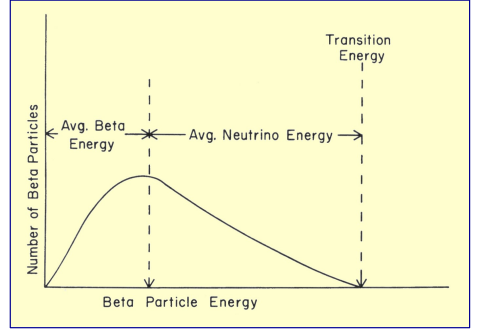
\includegraphics[scale=0.7]{Lezione9/fff.png} 
\end{figure}
Il risultato di questo è che il $Q$ valore è il valore finale di questa distribuzione di energia. Quindi non posso avere una energia maggiore del $Q$ valore. Corrisponde al caso in cui l'elettrone assorbe tuttta l'energia e il neutrino viene prodotto senza energia cinetica. Questo spettro si vede che ha $2$ zeri. Infatti vale zero se $p_e=0$ e viceversa vicino al $Q$ valore l'energia del neutrino è nulla. 

Per evidenziare l'effetto della correzione coulombiana questo è un caso di quelle curve corrispondeti ad $A$ pari in cui quello che dovrebbe essere un minimo della parabola è un nucleo dispari-dispari. Ma non è il minimo (non è stabile) perchè ha il termine aggiuntivo di energia dovuto al termine di pairing. Quindi questo qui è più alto in massa sia rispetto al nucleo che sta a destra sia al nucleo che sta a sinistra quindi può decadere in entrambi i modi. Andando a vedere lo spettro dei decadimenti $\beta$ ad esempio seguendo il decadimento $\beta^-$. L'elettrone viene attirato dal nucleo quindi il suo spettro è attirato a momenti bassi dell'elettrone. Invece guardando il decadimento $\beta^+$ viene emesso un positrone allora in questo caso la forza coulombiana è repulsiva ed infatti il punto zero non è praticamente popolato.  
%IMMAGINE rg
\begin{figure}[htp!]
  \centering
  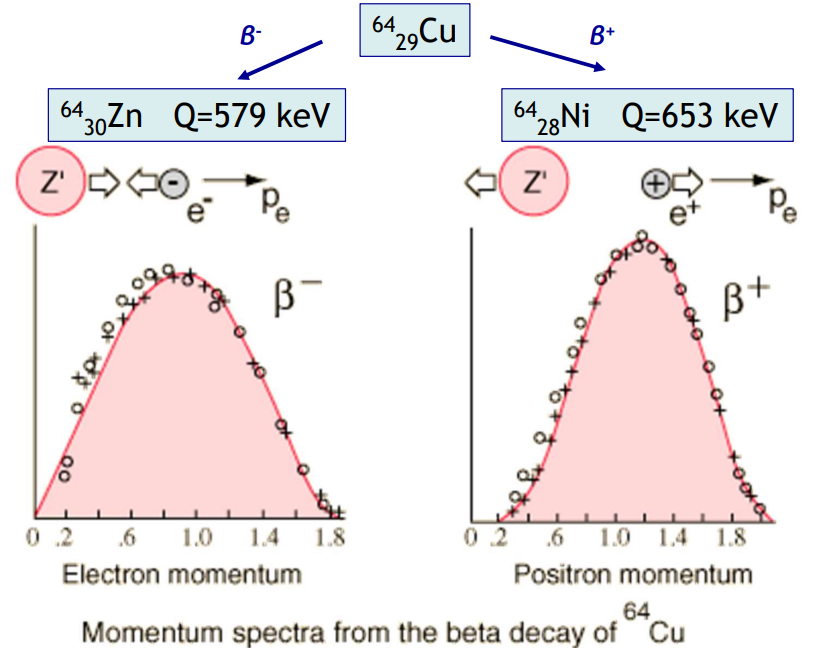
\includegraphics[scale=0.5]{Lezione9/rg.png} 
\end{figure}
Quindi se voglio calcolarmi la larghezza di decadimento totale devo fare l'integrale da il valore minimo dell'elettrone che è zero e il valore massimo che è il $Q$ valore. Quindi viene definito l'integrale adimensionale:
\begin{equation*}
    f(Z,Q)=\frac{1}{(m_ec^2)^5}\int_0^Qp_ec(T_e+m_ec^2)p_\nu E_\nu F(Z,T_e)dT_e
\end{equation*}
La probabilità:
\begin{equation*}
    \lambda=\frac{G_F^2(mc^2)^5}{2\pi^3\hbar}|M_{fi}|^2f(Z,Q)
\end{equation*}
Riassumento lo spazio delle fasi del decadimento in tre corpi dà la distribuzione differenziale di energia degli elettroni:
\begin{equation*}
    \frac{d\lambda}{dT_e}=\frac{G_F^2c^2}{2\pi^3\hbar}|M_{fi}|^2 p_e(T_e+m_ec^2)p_\nu E_\nu F(Z,T_e)
\end{equation*}
oppure:
\begin{equation*}
    \frac{d\lambda}{dp_e}=\frac{G_F^2c^4}{2\pi^3\hbar}|M_{fi}|^2p_e^2p_\nu E_\nu F(Z,T_e)
\end{equation*}
se $m_\nu=0,\,p_\nu cE_\nu=E_\nu^2=(Q-T_e)^2$
\begin{equation*}
    \frac{d\lambda}{dT_e}=\frac{G_F^2c^2}{2\pi^3\hbar}|M_{fi}|^2p_e(T_e+m_ec^2)(Q-T_e)^2F(Z,T_e)
\end{equation*}
e la larghezza totale è:
\begin{equation*}
    \lambda=\frac{G_F^2|M_{fi}|^2(m_ec^2)^5}{2\pi^2\hbar}f(Z,Q)
\end{equation*}
dove:
\begin{equation*}
    f(Z, Q)=\int_0^{Q / m_e c^2} d\left(\frac{T_e}{m_e c^2}\right) \frac{p_e}{m_e c}\left(1+\frac{T_e}{m_e c^2}\right)\left(\frac{Q-T_e}{m_e c^2}\right)^2 F\left(Z, T_e\right)
\end{equation*}
Nelle slide è possibile vedere come è stata misurata la massa del neutrino.
\subsection{Osservazione del neutrino}
Fino ad ora abiamo visto solo evidenza indiretta del neutrino, la prima rivelazione diretta del neutrino fu fatta da Reines e Cowan nel 1956. Utilizzarono la reazione di decadimento $\beta$ inverso:
\begin{equation*}
    \Bar{\nu}_e+p\to e^++n
\end{equation*}
La sorgente di antineutrini utilizzata fu un reattore nucleare. Abbiamo visto che in un reattore nucleare fra i prodotti della fissione ci sono emettitori $\beta$ a vita media breve. La cosa che aveva spaventato Pauli è stata che la sezione d'urto d'interazione di neutrini è molto piccola:
\begin{equation*}
    \sigma_{\Bar{\nu}p}\approx 5.6\frac{G_F^2E_\nu^2(\hbar c)^2}{\pi}
\end{equation*}
è relativamente facile costruire un bersaglio attivo di massa elevata che contiene protoni liberi (H). Possiamo compensare in due modi. Da una parte usando un reattore nucleare abbiamo un'eneorme quantità di fissioni e quindi di decadimenti $\beta$, quindi produciamo tanti antineutrini. Secondo posso avere un bersaglio con una massa molto elevata. Anche se la sezione d'urto è piccola il mio tasso di interezione rimane misurabile. [descrizione dell'esperimento delle slide]
\subsection{Spin isotopico}
Abbiamo visto che le interazioni nucleari sono identiche tra neutroni e protoni, differenza dovute alla interazioni elettromagnetiche. Possiamo assumere che per le interazioni forti esista una unica particella che può esistere in due stati: il nucleone $N$ che può trovarsi in due stati di carica, $p$ ed $n$. In pratica questo nucleone lo posso trattare come se avesse un altro grado di libertà interno come lo spin:
\begin{equation*}
    |p\rangle=\binom{1}{0} \qquad |n\rangle=\binom{0}{1}
\end{equation*}
\textbf{spin isotopico} $I$: $N$ ha $I=1/2$, ed i sue stati $p$ $I_3=+1/2$, $n$ $I_3=-1/2$. Segue delle regole di simmetria e di commutazione completamente analogo a quello dello spin. Questo grado di libertà interno, dovrebbe dare due stati degeneri perchè le interazioni forti vedono protoni e neutroni come uguali, non vedono lo spin isotopico. Questa degenerazione viene rotta dalla carica:
\begin{equation*}
    Q=\frac{A}{2}+I_3
\end{equation*}
Con $A$ numero di massa. Se si mette il protone e il neutrone effettivamente torna. Sistemi di nucleoni possono trovarsi in stati ben definiti di spin isotopico: se una certa hamiltoniana ha una simmetria possiamo sviluppare gli autostati della hamiltoniana come autostati della simmetria. I sistemi dei nucleoni possono essere classificati in base ai stati di spin isotopico ad esempio il deutone: esiste in un unico stato di carica I=0, composto da un neutrone e un protone. Essendo il nucleone un fermione (ha spin $1/2$) la funzione d'onda deve essere antisimmetrica. La funzione d'onda orbitale per $L=0,2$ è simmetrica, la funzione d'onda di spin per $S=1$ è simmetrica. Quindi la funzione d'onda di spin isotopico per $I=0$, è antisimmetrica:
\begin{equation*}
    \frac{1}{\sqrt{2}}( |p\rangle|n\rangle-|n\rangle|p\rangle)
\end{equation*}
Ed è per questo che il deutone può essere in un solo stato di carica. Questo è un modo diverso per dire perchè non esistono nuclei con solo due neutroni o solo due protoni. Infatti con il momento angolare pari, lo spin $=1$ lo spin isotopico deve per forza essere uguale a $=0$.
%IMMAGINE es
\begin{figure}[htp!]
  \centering
  
\includegraphics[scale=0.4]{Lezione9/es.png} 
\end{figure}
Nel primo esempio i due sistemi di nucleoni in due stati di spin isotopico diversi sono uguali ma differiscono tra l'ultimo livello dove nel primo c'è il protone, nel secondo il neutrone (questi due stati sono detti doppietto di spin isotopico). Sono distinguibili solo grazie alla interazione elettromagnetica. Per quanto riguarda lo spin-sparità è esattamente identico, le masse differiscono di poco e dalla differenza di massa si stima il terzo termine della formula di Bethe Weizs\"aker. Un caso più complicato è quando ho due nucleoni che "ballano". Avendo due particelle che possono avere spin isotopico $1/2$ e $-1/2$ le posso combinare ottenendo $I=1$ o $I=0$. Questo accade con $A=14$. I primi due livelli sono pieni e a seconda dei numeri di nucleoni posso avere combinazioni diverse. Lo stato fondamentale è quello più a destra, se però prendiamo il primo stato eccitato del'azoto-14 scopriamo di avere spin-parità nullo. La differenza di eccesso di massa riflettono la repulsione coulombiana infatti tutto a sinistra avendo due protoni ho una massa maggiore di quando ho un protono e un neutrone o addirittura due neutroni. Quello con eccesso di massa minore però è quello con un neutrone e un protone. Questi stati decadrebbero nello stato con energia (massa minore). La cosa interessante è che quando abbiamo dei nuclei che sono tra di loro in un doppietto di spin isotopico. Le trasformazioni e i decadimenti $\beta$ li possiamo trattare come operatori di innalzamento e abbassamento dell'operatore spin isotopico $I_\pm$ questo funziona masse abbastanza basse. Per $A$ grande abbiamo un sbilanciamento importante, aumentando $A$ il numero di neutroni aumenta rispetto al numero di protoni per la repulsione elettrostatica. Questa enorme differenza rompe completamente la degenerazione. Quindi ovviamente per avere doppietto isotopico bisogna avere protone e neutrone nello stesso livello energetico.
\subsection{Determinazione della costante di Fermi}
Nella maggior parte dei casi, si usa il tempo di decadimento per stimare l'elemento di matrice. Infatti misuro in qualche modo la costante di fermi e successivamente trovo l'elemento di matrice. Per misurare la costante di fermi però devo trovare un decadimento in cui conosco l'elemento di matrice. Ci sono dei decadimenti particolari in cui per ragioni di simmetria si può valutare con precisione $M_{fi}=\sqrt{2}$. Sono tutti decadimenti $\beta^+$, tra elementi di un tripletto di spin isotopico con $J^\pi=0$. In questi casi gli operatori di innalzamento e abbassamento agiscono:
\begin{equation*}
    I_{-}\left|I=1, I_3=+1\right\rangle=\sqrt{2}\left|I=1, I_3=0\right\rangle, \quad I_{-}\left|I=1, I_3=0\right\rangle=\sqrt{2}\left|I=1, I_3=-1\right\rangle
\end{equation*}
Sono sempre in competizioni con cattura elettronica o altri stati finali:
\begin{equation*}
    \Gamma=\frac{1}{\tau}\frac{\text{BR}}{1+P_{EC}}
\end{equation*}
Questa larghezza di decadimento che mi calcolo dalla regola d'oro di Fermi. Quindi $1/\tau$ è il $\Gamma_{totale}$ mentre il BR è la frazione di decadimenti $\beta:\,\,0^+\to0^+$. Mentre $P_{EC}$ è la frazione di decadimenti per $EC$. Bisogna fare un pochino di attenzione in quanto non basta prendere una costante di decadimento per il decadimento $\beta$ ma bisogna andare a prendere specificatamente quel decadimento con stato iniziale e stato finale $0^+$.

Infine, invece della vita media, è tradizione usare il tempo di dimezzamento:
\begin{equation*}
    t_{1/2}=\tau\ln{2}
\end{equation*}
La costante di Fermi nel decadimento $\beta$ si ricava dunque a partire dal valore misurato $ft$:
\begin{equation*}
  ft=f(Z, Q) \frac{t_{1 / 2}}{B R}\left(1+P_{E C}\right)=\frac{\ln 2 \pi^3 \hbar}{G_F^2\left(m_e c^2\right)^5}
\end{equation*}
Guardando la tabella dei decadimenti super-permessi si nota che la $f$ varia di svariati ordini di grandezza. Anche il tempo di dimezzamento ma per questi decadimenti il prodotto è circa costante. Giustificando che l'elemento di matrice è uguale per tutti. 
\begin{equation*}
    G_F=(1.14962\pm0.00015)\times 10^{-5}\,GeV^{-2}
\end{equation*}
\subsection{Riassumendo}
Nel decadimento $\beta$, un elettrone ed un neutrino vengono prodotti \textbf{all'interno del nucleo}. Molto importante in quanto prima non ci sono e vengono creati proprio durante questo processo. Cinematicamente il nucleo bilancia il momento ricevendo sempre poca energia. La prima teoria di fermi del decadimento $\beta$: interazione di contatto. Calcolando la probabilità di decadimento della "regola d'oro" e si è calcolata la costante dell'intensità di interazione. Nei decadimenti "permessi" l'elemento di matrice non dipende (in prima approssimazione) dal momento di elettrone e neutrino. Lo spettro del decadimento viene descritto completamente dal \textbf{termine di spazio delle fasi}. In alcune transizione l'elemento di matrice è quasi calcolabile: concetto di spin isotopico (o isospin) e misura della costante di Fermi. Prime proprietà del neutrino $m_\nu<1.1\,eV$.